\documentclass[border=4pt]{standalone}
\usepackage{fontspec}
\usepackage{amsmath}
\usepackage{unicode-math}
\setmainfont{Latin Modern Roman}
\setmathfont{Latin Modern Math}
\usepackage{pgfplots}
\usepackage{pgfplotstable}
\pgfplotsset{compat=1.18}
\usepackage{tkz-euclide}
\usetikzlibrary{arrows.meta,calc,angles,quotes,patterns,3d,backgrounds}
\definecolor{ink}{HTML}{123428}
\definecolor{asy}{HTML}{475569}
\definecolor{mint}{HTML}{86e0bd}
\tikzset{asym/.style={asy, line width=0.9pt, dash pattern=on 5pt off 3.5pt},
         guide/.style={gray!70, line width=0.6pt, densely dotted},
         dot/.style={circle, inner sep=0pt, minimum size=5pt, draw=white, line width=0.5pt},
         odot/.style={circle, inner sep=0pt, minimum size=5.5pt, fill=white, line width=1pt},
         lab/.style={font=\footnotesize, inner sep=1.5pt, text=ink}}
\begin{document}
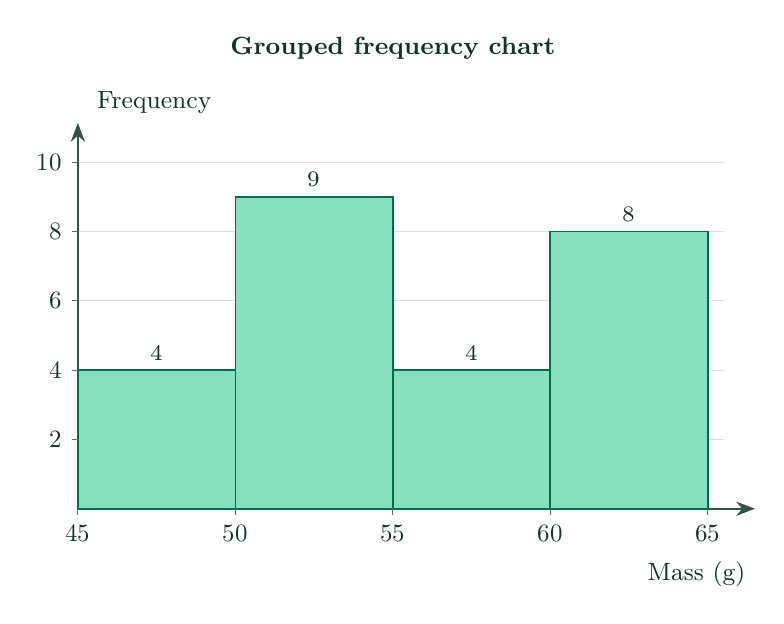
\begin{tikzpicture}
\draw[gray!25, line width=0.4pt] (0,0.880) -- (8.200,0.880);
\draw[gray!25, line width=0.4pt] (0,1.760) -- (8.200,1.760);
\draw[gray!25, line width=0.4pt] (0,2.640) -- (8.200,2.640);
\draw[gray!25, line width=0.4pt] (0,3.520) -- (8.200,3.520);
\draw[gray!25, line width=0.4pt] (0,4.400) -- (8.200,4.400);
\draw[ink!85, line width=0.7pt, -{Stealth[length=2.4mm]}] (0,0) -- (8.600,0);
\draw[ink!85, line width=0.7pt, -{Stealth[length=2.4mm]}] (0,0) -- (0,4.900);
\draw[draw={rgb,255:red,4;green,107;blue,77}, fill={rgb,255:red,134;green,224;blue,189}, line width=0.6pt] (0.000,0) rectangle (2.000,1.760);
\node[font=\footnotesize, text=ink, above] at (1.000,1.760) {$4$};
\draw[draw={rgb,255:red,4;green,107;blue,77}, fill={rgb,255:red,134;green,224;blue,189}, line width=0.6pt] (2.000,0) rectangle (4.000,3.960);
\node[font=\footnotesize, text=ink, above] at (3.000,3.960) {$9$};
\draw[draw={rgb,255:red,4;green,107;blue,77}, fill={rgb,255:red,134;green,224;blue,189}, line width=0.6pt] (4.000,0) rectangle (6.000,1.760);
\node[font=\footnotesize, text=ink, above] at (5.000,1.760) {$4$};
\draw[draw={rgb,255:red,4;green,107;blue,77}, fill={rgb,255:red,134;green,224;blue,189}, line width=0.6pt] (6.000,0) rectangle (8.000,3.520);
\node[font=\footnotesize, text=ink, above] at (7.000,3.520) {$8$};
\draw[ink!70] (0.000,0) -- (0.000,-0.08) node[below, font=\small, text=ink] {$45$};
\draw[ink!70] (2.000,0) -- (2.000,-0.08) node[below, font=\small, text=ink] {$50$};
\draw[ink!70] (4.000,0) -- (4.000,-0.08) node[below, font=\small, text=ink] {$55$};
\draw[ink!70] (6.000,0) -- (6.000,-0.08) node[below, font=\small, text=ink] {$60$};
\draw[ink!70] (8.000,0) -- (8.000,-0.08) node[below, font=\small, text=ink] {$65$};
\draw[ink!70] (0,0.880) -- (-0.08,0.880) node[left, font=\small, text=ink] {$2$};
\draw[ink!70] (0,1.760) -- (-0.08,1.760) node[left, font=\small, text=ink] {$4$};
\draw[ink!70] (0,2.640) -- (-0.08,2.640) node[left, font=\small, text=ink] {$6$};
\draw[ink!70] (0,3.520) -- (-0.08,3.520) node[left, font=\small, text=ink] {$8$};
\draw[ink!70] (0,4.400) -- (-0.08,4.400) node[left, font=\small, text=ink] {$10$};
\node[font=\small, text=ink, anchor=north east] at (8.600,-0.55) {Mass (g)};
\node[font=\small, text=ink, anchor=south west] at (0.12,4.900) {Frequency};
\node[font=\bfseries\small, text=ink] at (4.000,5.850) {Grouped frequency chart};
\end{tikzpicture}
\end{document}
